\documentclass[thesis.tex]{subfiles}
\begin{document}
\chapter{Future Work}
\label{chap:future-work}

So far we have described the policies of the mobile ecosystem and how AppPAL can
be used to describe them. We have argued that AppPAL is a good language for
describing these policies, however there are also areas where AppPAL could be
improved to further to describe more kinds of policies and to aid policy
authors, as well as examining further aspects of the mobile ecosystem. This chapter
suggests several areas which we did not look at and why they might offer an
interesting insight into mobile ecosystems. We also describe how plausibility,
quantified doubt, could be used to express confidence in a statement in an
AppPAL policy.


\section{Plausible SecPAL}

The SecPAL authorization language, and the AppPAL instantiation, allow
policy authors to make use of static analysis tools to make decisions,
and allow principals to make statements about apps through delegation.
When these decisions are made they are made with certainty.  If a
principal says an app is safe to access the network then we believe
that that principal definitely believes the app is safe on a network.
When a static analysis tool finds that an app isn't malware then we
believe that app to not be malware.  This isn't realistic.  Static
analysis tools can produce false results.  A principal might be merely
fairly confident that an app can access the network safely but not absolutely
certain.

With current authorization languages you cannot quantify the belief a principal
has in any statement. A principal cannot say how \emph{plausible} they think any
statement is.

\subsection{Examples of Plausibility}

SecPAL was designed to make access control decisions. The decision whether to
install allow a user access to a file or not is a binary one: either they can
access it or they cannot. Similarly the decision process for these decisions is
also binary: a user is either logged in or not, a network address is either in
the network or outside it, someone can act as someone else's manager or they can
not. Not all decisions are binary however.

\begin{figure}
  \centering
  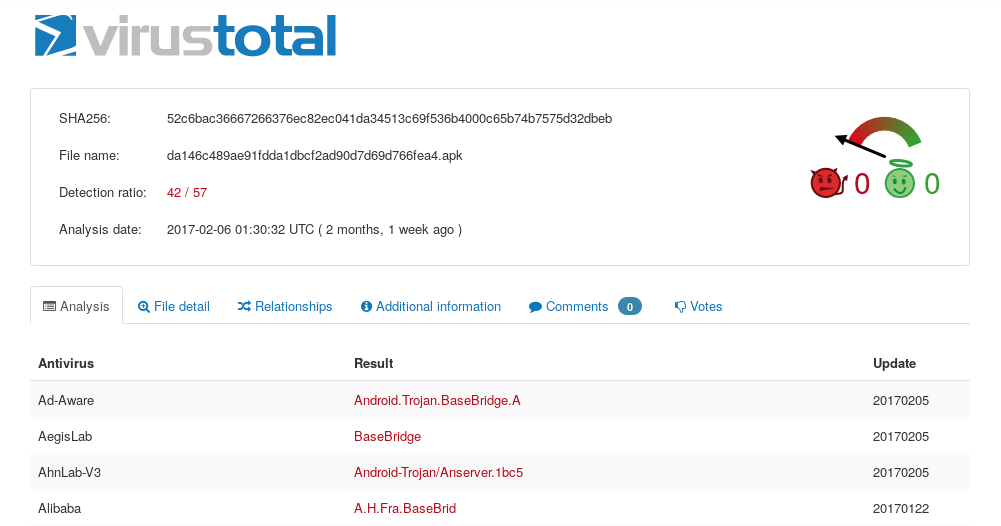
\includegraphics[width=0.49\linewidth]{figures/android-malware.png}
  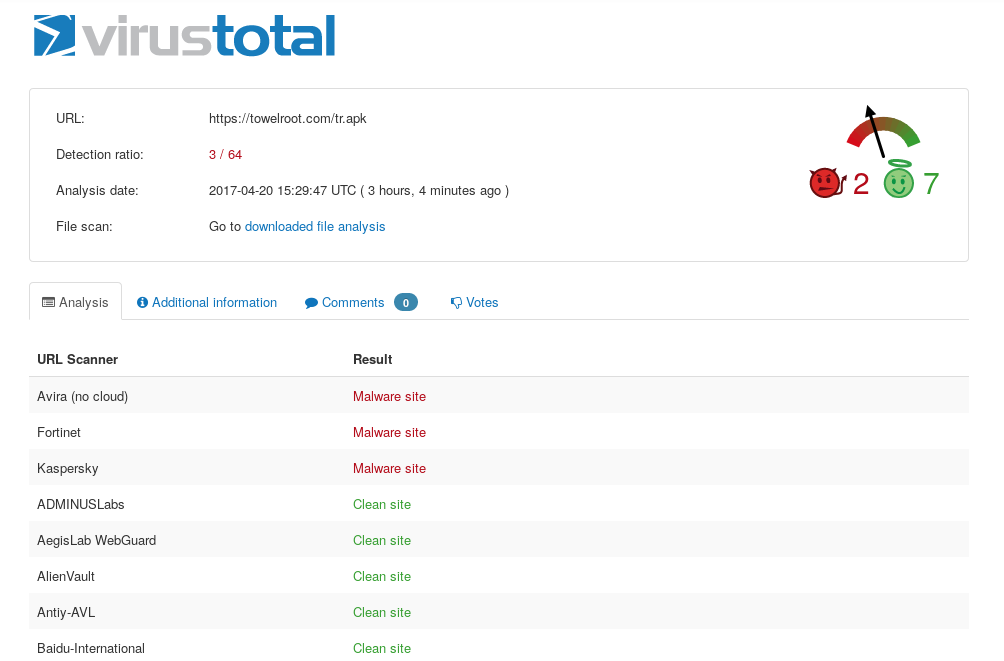
\includegraphics[width=0.49\linewidth]{figures/towelroot.png}
  \caption[VirusTotal results for two Android apps.]{VirusTotal results for 57
    antivirus packages scanning a sample of the BaseBridge Android malware, and 64
    antivirus packages analyzing a download of the (relatively safe) Towelroot
    rooting app.}
  \label{fig:android-malware}
\end{figure}

A user, Alice, may have a policy. That will only install safe apps, ones they
know are not malware. She could use an \ac{AV} program, but these tools are not
infallible. Some change their mind about apps over time. Others are heuristic
based and may only be capable of judging an app based on sufficiently many
malware indicators being present. Instead of using one \ac{AV} program, Alice
opts to use \emph{VirusTotal}; a webservice for running files through multiple
\ac{AV} programs. Even for known malware samples VirusTotal rarely gives
absolute answers instead giving the number of \ac{AV} programs that flagged
it~(\autoref{fig:android-malware}). Alice acknowledges this and writes her
policy accordingly:

\begin{lstlisting}
'alice' says App:A isInstallable
  if A isSafe
  with plausibility at least 0.75.

'alice' says 'virustotal' can-say
  App:A isSafe

'virustotal' says 'com.good.app' isSafe
  with plausibility 0.95.

'virustotal' says 'com.malicious.app' isSafe
  with plausibility 0.26.
\end{lstlisting}

She can install the \texttt{com.good.app}, since the plausibility it is good is
greater than her threshold but the \texttt{com.malicious.app} fails her test and
is uninstallable. 

In the first example VirusTotal gave Alice a value for how plausible it was the
app was safe: but what if Alice has to decide this value herself? An example of
this is app recommendations. Alice only wants to install apps that are really
good. She has two friends, Bob and Charlie, who offer her reviews of a game. To
complicate matters further, whilst she trusts Bob utterly, she is a little less
trusting of Charlie.

\begin{lstlisting}
'alice' says App:A isInstallable
  if A isGood
  with plausibility

'bob' says 'com.rovio.angrybirds' isGood
  with plausibility 0.8.

'charlie' says 'com.rovio.angrybirds' isGood
  with plausibility 0.9.

'alice' says 'bob' can-say App:A isGood.

'alice' says 'charlie' can-say App:A isGood
  with plausibility 0.9.
\end{lstlisting}

How should she combine the information to get an overall rating of the game? If
Alice wants to only install an apps that are both good and safe how should she
trade off the plausibility against each other? Is she willing to install a more
dangerous app if it is highly reviewed?

Plausibility is similar to probability (plausibility incorporates the speakers
\emph{belief} that the statement is true as opposed to just its likelihood) and
various papers have proposed probabilistic variants of
Datalog~\cite{fuhr_probabilistic_1995} or explored the semantics of
probabilistic logics~\cite{halpern_analysis_1990}. Role-based access control
languages have incorporated ideas about risk into their
schemes~\cite{josang_analysing_2004,dimmock_using_2004,salim_approach_2011},
which is a similar notion to plausibility and trust. These schemes do not seem
to deal with delegation in the same manner as SecPAL however so incorporating
similar ideas here may be interesting and allow SecPAL and AppPAL greater
expressiveness..

\subsection{Guarantees for Plausible SecPAL} 

In \autoref{appendix:probabilistic} we suggest how we might implement Plausible
SecPAL by modifying Becker~\etal's original design. However we implement it, we
should consider carefully how we might \emph{combine} information and
plausibilities. Combining probabilities of events when you cannot guarantee
independence is hard, and the same is true of plausibility. Simple strategies
such as taking the product, minimum or maximum of combined statements are simple
solutions, though better ones undoubtably exist. However plausibility
combination is implemented some thought should be given to what properties and
guarantees Plausible SecPAL ought to offer. We suggest the following:

\begin{enumerate}
\item \label{enum:1} If all facts are completely plausible, then evaluation should be
  equivalent to standard SecPAL.
\item \label{enum:0} If any fact is completely  implausible, then it should be equivalent
  to the statement not existing in the assertion context.
\item \label{enum:grow} No derived statement should be more plausible than the conditions used
  to derive it.
\end{enumerate}

Rule~\ref{enum:1} ensures that any plausibility additions do not start to
produce different results to standard SecPAL. We wish to be able to reason about
scenarios where we have partial plausibility, but this addition shouldn't change
our ability to reason when each speaker has total belief in their assertions. If
everything is completely plausible, then the reasoning should be equivalent to
SecPAL where the perfect plausibility is assumed. Similarly if a speaker
believes a fact to be completely implausible then Rule~\ref{enum:0} ensures that
fact is used to derive other facts. SecPAL operates under a \emph{closed world
assumption}, that is that the assertion context contains (or at least can
derive) \emph{all} known facts. If a statement is missing then it is false. If a
speaker believes a statement to be perfectly implausible then it should be
equivalent to falsehood in standard SecPAL and should not be used further.

Rule~\ref{enum:grow} applies to assertions with a conditional part (i.e.~an
\texttt{if}). If this rule were not the case we might be able to grow the
plausibilty of a fact by applying a rule that contained its own derived fact in
its condition. For example consider the following rule:
\begin{lstlisting}
'x' says 'y' p
  if 'y' p,
     'z' q.
\end{lstlisting} Say we know already that by applying this rule the plausibility
that \texttt{'x' says 'y' p} will be greater than the plausibility of the
conditionals that \texttt{'x' says 'y' p} and \texttt{'x' says 'z' q}. Since the
decision that \texttt{'x' says 'y' p} is also part of the conditions, we could
repeatedly reapply this rule and raise the plausibility arbitrarily.


\section{Other Markets}

There are many different markets available for Android, each with their own
policies and apps within them. In~\autoref{chap:apps-and-stores} we looked at
the policies four different stores as well as Apple's store and started to make
comparisons. The stores we looked at, however, were all common to Europe, Russia
and the US.

Other marketplaces, of course, exist. In particular the app ecosystem in China
appears to be somewhat different as it has grown independently of Google. We did
not examine these markets extensively, however, describing the differences
between these stores and the western ones would make for an interesting
comparison. One particularly interesting area might be to look at the apps sold.
In all the stores we looked at many of the same apps appeared on the stores
front pages. The Chinese stores have completely different sets of apps. Building
a precise description of the different sets of apps each region uses would allow
us to contrast what users are doing with their devices (i.e.~playing games,
work, video) as well as which companies are collecting their data.

\section{AppPAL Enforcement and Usability}

We have shown in this dissertation how AppPAL can be used to describe different
policies for BYOD, and for app installation preferences. A logical next step
would be to start to use AppPAL to enforce these policies, and to study how
users might use AppPAL to make decisions.

One way of doing this might be to use AppPAL as a mechanisms for finding apps
that match user's privacy policies. We described earlier how we could use
AppPAL's \emph{genstore}-framework to build a curated app store on the basis of
a policy. This could be extended to allow for app searches. AppPAL is designed
to be readable, but we might guess that most non-technical users would struggle
with writing a formal policy (as they do with many other technical tasks).
Exploring how general users might use policies, either through a subscription
model where they \emph{subscribe} to a policy written by a more advanced user,
or through a graphical interface that helps them build their own policy, would
help us understand how (and infact whether at all) user's want to use better app
controls. 

BYOD is another area where it would be interesting to see how AppPAL might be
used in practice. When talking about BYOD policies we said that AppPAL was
designed to separate the policy specification from its implementation. By
combining AppPAL policies with an MDM package we could dynamically configure the
MDM software to enforce a BYOD policy. This could allow for greater
customization as not only could we extend the simplistic MDM policy setting with
a full policy language. Trialing an implementation in a company and working with
the IT departments and policy authors to better understand their needs would
allow us to tailor AppPAL further to implementing BYOD policies.




\end{document}

%%% local variables:
%%% mode: latex
%%% tex-master: "../ch6.tex"
%%% end:
